\chapter{Implementation}

In this chapter we will describe the implementation details of the MeshDiff program. We will explain how triangle meshes are represented in the program and we will talk about the following three steps of the visualization algorithm:

\begin{itemize}
\item Difference metric computation
\item Data point clustering
\item Data point visualization
\end{itemize}

We will also mention how the algorithm is incorporated into MeshDiff, how mesh viewing works and how the user interface is designed to support the features outlined in section \ref{sec:meshdiff_features}.

%%-----------------------------------------------------------------------------------------
%% SECTION
%%-----------------------------------------------------------------------------------------
\section{Visualization Algorithm}

The core class of MeshDiff which encapsulates the visualization algorithm is called \verb+DiffVector+. The name of the class suggests that it is able to work with difference metrics which can be represented by a vector, more specifically a 3D vector. \verb+DiffVector+ is initialized by data of the two meshes to be compared and therefore only operates on these two specific meshes throughout its whole lifetime.

The main public methods of \verb+DiffVector+ are \verb+CreateVisualization()+ and \verb+BakeVisualization()+. \verb+CreateVisualization()+ is responsible for metric computation, data point clustering and the generation of a visualization. This visualization is then stored inside the \verb+DiffVector+ class and can be obtained by copying it into an output triangle mesh in the \verb+BakeVisualization()+ method.

This approach ensures that all intermediate results which are difficult to compute like data point clustering and visualization data can be stored inside the \verb+DiffVector+ class and quickly retrieved later if necessary. When a new visualization is created on the same pair of meshes, all intermediate results which can be reused are reused and only the ones which change are computed.

The fact that visualizations are outputted in the form of triangle meshes makes it easy to display, load and store the visualizations using standard triangle mesh methods and formats.

We will now present all steps of the visualization process in more detail.

%%-----------------------------------------------------------------------------------------
\subsection{Triangle Mesh Representation}
\label{sec:mesh_representation}

We are using the implementation of a boundary representation of a triangle mesh with a corner table which was presented in \citet{Corner03}. The implementation was created by Josef Pelikán. For brevity, we will refer to this representation as a {\it scene representation}\footnotemark.

\footnotetext{In this representation, we do not store the vertices of the triangle mesh but the corners of the triangles. Corner table then allows us to obtain the neighboring as well as opposite corners of a given corner and associated vertices in constant time. This makes traversing an arbitrary triangle mesh very simple and fast.}

We have added several methods to this implementation in order for us to be able to quickly obtain the list of neighbors of a given vertex and compute the geometrical area of clusters.

%%-----------------------------------------------------------------------------------------
\subsection{Difference Metric Computation}
\label{sec:analysis_metric}

This step of the visualization process can be configured by a parameter passed to the \verb+CreateVisualization()+ method. \verb+DiffVector+ remembers the current metric which it has computed and this determines whether it will be reused or whether a new one will be computed.

As mentioned earlier, we have included two difference metric in MeshDiff, both of which can be represented by a 3D vector:

\begin{itemize}
\item Corresponding vertex distance
\item Corresponding vertex distance projected into the surface normal
\end{itemize}

We have created a common representation for for both of these metrics called \verb+Arrow+ which acts as a data point, an input to the clustering algorithm.

Here are the most important fields of an \verb+Arrow+:

\begin{itemize}
\item Origin - a 3D vector representing the position of the vector metric and initially coincides with the coordinates of the corresponding vertex
\item Direction - a 3D vector representing the metric itself
\item Orientation - tells whether the arrow points "inside" or "outside" the triangle mesh or if the orientation is unknown
\end{itemize}

During this step, all corresponding vertices of both meshes are enumerated and for each pair, a corresponding metric is computed using the {\it scene representation}.

\subsubsection{Output}

A list of \verb+Arrow+ instances indexed by the handles of the corresponding vertices in the {\it scene representation}.

%%-----------------------------------------------------------------------------------------
\subsection{Data Point Clustering}
\label{sec:implementation_clustering}

As mentioned in \ref{sec:analysis_clustering_algorithm}, our clustering has multiple types. For the sake of consistency, we also introduce a third type, the empty clustering, which does not reduce the number of data points in any way and can be used when no clustering is needed. Each clustering type has an associated class, all of which share a common interface.

The clustering type used in \verb+DiffVector+ is determined by a factory method passed its constructor. \verb+DiffVector+ can therefore use the clustering without knowing its type and at the same time it is limited to using only one clustering type. Thanks to this, computed clusterings can be saved and reused if needed. It is important to note that this reuse happens every time the user chooses to view a new visualization which differs from the previous one only in the number of clusters to be used. The parameters of the clustering are then passed directly to the \verb+CreateVisualization()+ method.

The clustering object converts the \verb+Arrow+ instances (data points) to \verb+Cluster+ instances which are able to merge with other clusters and compute the clustering error given another \verb+Cluster+ instance. They also contain all the information needed for the visualization to be created. Here are their most important fields:

\begin{itemize}
\item Neighbors - a set of \verb+Cluster+ instances adjacent to the cluster
\item Level - marks the step of the clustering algorithm in which this cluster was created (low number also means low clustering error)
\item Representative Arrow - an \verb+Arrow+ instance representing the metric value for this cluster
\item Size - the geometrical area of the cluster
\item Left Child \& Right Child - \verb+Cluster+ instances out of which this cluster was created
\item Primary Data Points - a list of all the original unclustered data points which are tied directly to the underlying mesh and which belong to this cluster
\end{itemize}

\verb+Cluster+ instances can be sorted according to their level.

In general, each clustering object is initialized by the \verb+DiffVector+ class with a list of \verb+Arrow+ instances from the previous step (\ref{sec:analysis_metric}). Then \verb+DiffVector+ passes clustering parameters and the required cluster count to the clustering object. The clustering object checks if it already has a clustering corresponding to the given parameters and if it does, it simply extracts the required number of clusters from the available dendrogram and returns them. This is how the extraction works when the dendrogram is a tree\footnote{In this case, merging candidates only have to be neighbors}:

\begin{algorithm}[H]
\caption{Cluster Extraction from a Tree}
\begin{algorithmic}[1]

\Require MaxHeap chosenClusters, requiredClusterCount
\Statex
\State chosenClusters.Clear();
\State chosenClusters.Insert(dendrogram root);
\State i = 0;
\While{i < requiredClusterCount}
	\State highestCluster = chosenClusters.ExtractMax();
    \State chosenClusters.Insert(highestCluster.LeftChild);
    \State chosenClusters.Insert(highestClusters.RightChild);
    \State i++;
\EndWhile
\Statex
\Return chosenClusters as list
\end{algorithmic}
\end{algorithm}

Here is the extraction algorithms for forest dendrograms\footnote{In this case, merging candidates have to be neighbors and their vectors must point in the same direction}:

\begin{algorithm}[H]
\caption{Cluster Extraction from a Forest}
\label{algo:extraction_forest}
\begin{algorithmic}[1]

\Require MaxHeap chosenClusters, requiredClusterCount
\Statex
\State chosenClusters.Clear();
\State chosenClusters.Insert(all dendrogram roots);
\State i = 0;
\While{i < requiredClusterCount}
	\State highestCluster = chosenClusters.ExtractMax();
    \State chosenClusters.Insert(highestCluster.LeftChild);
    \State chosenClusters.Insert(highestClusters.RightChild);
    \State i++;
\EndWhile
\State list = chosenClusters.ExtractMaxNTimes(requiredClusterCount);
\Statex
\Return list
\end{algorithmic}
\end{algorithm}

Line 9 of algorithm \ref{algo:extraction_forest} makes sure that clusters which were chosen only because they are roots (line 2) and not because their level is high enough are excluded from the selection.

If the desired clustering is not available, the clustering object performs the clustering algorithm. Here is the outline of it (largely similar to the one in \citet{Telea99}):

\begin{algorithm}[H]
\caption{Clustering}
\begin{algorithmic}[1]

\Require dataPoints, initalClusters, MinHeap clusteringCandidates \Comment clusteringCandidates are ordered by clustering error
\Statex
\For{each point\textsubscript{i} \textbf{in} dataPoints}
	\State initialCluster = makeCluster(point\textsubscript{i});
    \State set level of intialCluster to 0;
    \State add initialCluster to initialClusters;
\EndFor
\Statex
\For{each cluster\textsubscript{i} in initialClusters}
	\For{each cluster\textsubscript{j} neighbour of cluster\textsubscript{i}}
    	\State e = clusteringError(cluster\textsubscript{i}, cluster\textsubscript{j});
        \State insert (cluster\textsubscript{i}, cluster\textsubscript{j}) into clusteringCandidates
        \State mark cluster\textsubscript{i} and cluster\textsubscript{j} as NOT\_CLUSTERED;
    \EndFor
\EndFor
\Statex
\State level = 0;
\While{clusteringCandidates.Count > 0}
	\State (cluster\textsubscript{i}, cluster\textsubscript{j}) = clusteringCandidates.ExtractMin();
    \If{cluster\textsubscript{i} and cluster\textsubscript{j} are both NOT\_CLUSTERED}
    	\State newCluster = mergeClusters(cluster\textsubscript{i}, cluster\textsubscript{j});
        \State set level of newCluster to level++;
		\State mark newCluster as NOT\_CLUSTERED;
        \State mark cluster\textsubscript{i} and cluster\textsubscript{j} as CLUSTERED;
        \For{each cluster neighbour of newCluster}
        	\State e = clusteringError(cluster, newCluster);
            \State insert (cluster, newCluster) into clusteringCandidates
        \EndFor
    \EndIf
\EndWhile
\Statex
\Return c as root of tree
\end{algorithmic}
\end{algorithm}

It is worth mentioning that when a new cluster is created, it needs to be placed in the clustering space by assigning all neighboring clusters of its two children to be the neighbors of the new cluster as well, except for the children themselves. Also, the neighboring relation has to be made symmetrical by updating the neighbor lists of the surrounding clusters as well.

\subsubsection{Output}

A list of \verb+Cluster+ instances is returned, even in the case of empty clustering where the only operation is the conversion of \verb+Arrow+ instances into \verb+Cluster+ instances.

%%-----------------------------------------------------------------------------------------
\subsection{Data Point Visualization}

In section \ref{sec:analysis_visualizations}, we have proposed several types of visualizations. Each of them has an associated class in MeshDiff which generates it based on \verb+Cluster+ instances supplied to it. There are two interfaces which these visualizer classes can implement, depending on whether they produce arrow-based or color-based visualizations. Objects of these classes are passed to the \verb+CreateVisualization()+ method which stores the visualizations in the \verb+DiffVector+ object. Because arrow-based and color-based visualizations can be combined into one, \verb+CreateVisualization()+ accepts two visualizer parameters, one for each interface. At least one of them should be provided for the \verb+DiffVector+ class to generate a visualization.

We will now focus on the visualizers of the two interfaces separately.

\subsubsection{Arrow Visualizers}

Arrow visualizer objects only have one field which is initialized in the constructor. This field hold a basic triangle mesh representing a 3D arrow. This arrow was created manually in order to have the least amount of vertices and triangles possible. It has 17 vertices and 16 triangles. The tip of the arrow is an eight-sided pyramid which has a much better appearance than the basic four-sided pyramid.

\begin{figure}[h]
\centering
	\begin{subfigure}{0.3\textwidth}
	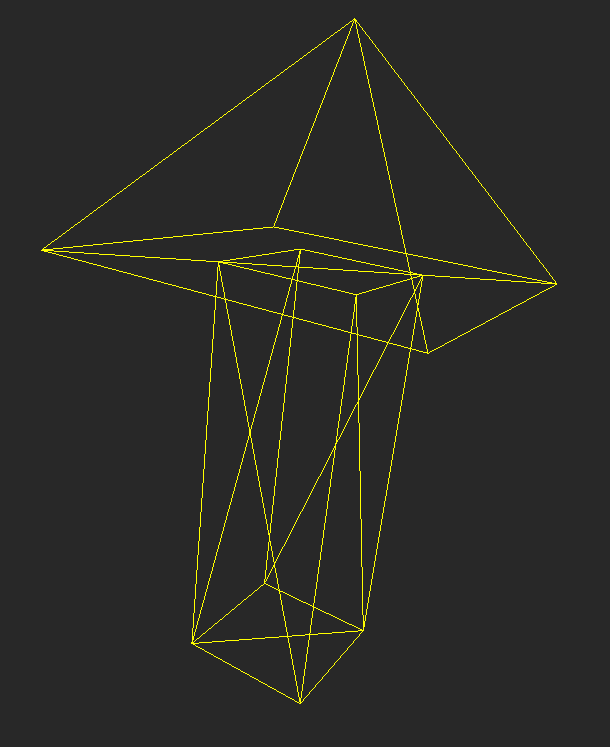
\includegraphics[width=\textwidth]{./img/4sided_arrow.PNG}
    \caption{Four-sided tip version (not used)}
    \label{fig:4sided_arrow}
	\end{subfigure}
    \qquad
    \begin{subfigure}{0.3\textwidth}
	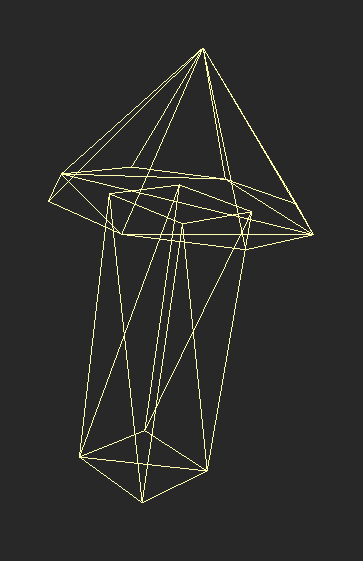
\includegraphics[width=\textwidth]{./img/8sided_arrow.PNG}
    \caption{Eight-sided tip version (used)}
    \label{fig:8sided_arrow}
	\end{subfigure}
\caption{Wireframe models used for arrow visualizations}
\end{figure}

The visualizer receives a list of clusters as input, loops through them and makes a scaled copy of the basic arrow in each iteration. The scale of the copy is based on the representative vector of the cluster as described in section \ref{sec:analysis_visualizations}. An output triangle mesh containing all the created copies is then outputted.

\subsubsection{Color Visualizers}

For each mode mentioned in section \ref{sec:analysis_visualizations} (i.e. random, cluster relative, cluster absolute, etc.), there is a separate visualizer class implementing the color visualizer interface. This determines how color is assigned to vertices. In general, each visualizer loops though all clusters supplied and for each of them it generates a color based on the metric value for that cluster. Once a color is created, it is inserted into a list at precisely those indices which belong to the primary data points (see section \ref{sec:implementation_clustering}) of the associated cluster in the {\it scene representation} of the underlying triangle mesh. It is important to respect this indexing in order to make the mapping of the colors to the mesh vertices easier in the \verb+BakeVisualization()+ method of the \verb+DiffVector+ class. This list is then outputted.

\subsubsection{Output}

Either a triangle mesh or a list of triplets representing colors is outputted based on the type of the visualization.
%%-----------------------------------------------------------------------------------------
%% SECTION
%%-----------------------------------------------------------------------------------------
\section{MeshDiff Architecture}

When introducing the design of MeshDiff, we will first discuss the original code by Josef Pelikán used for mesh viewing and how we modified it, then we will describe how the user interface has been changed to support features outlined in section \ref{sec:meshdiff_features} and then we will show how the visualization algorithm has been incorporated into the program.

%%-----------------------------------------------------------------------------------------
\subsection{Triangle Mesh Viewing}

The original code of MeshDiff support the two most common standard triangle mesh formats, \verb+.obj+ and \verb+.ply+. It is able to load and store files of these formats and also convert between them and the internal representation (see section \ref{sec:mesh_representation}) of a triangle mesh. This {\it scene} can then be rendered by calling its own method which fills the vertex buffer object with its data. In each frame, a special rendering method is called which comprises OpenTK calls tied to a WinForms control showing the triangle mesh. This process can be modified by a set of toggles which can change the viewing mode to wireframe or turn on shading.

Interactivity is handled by a class called \verb+Trackball+ which intercepts mouse clicks and moves from the user interface and modifies the model matrix used in the rendering process.

We have generalized this process slightly for the purpose of showing two triangle meshes at the same time. We have doubled the number of buffer objects and added parameters to the rendering methods which allow us to choose which {\it scene} to render and where to render it. Each viewing panel has its own \verb+Trackball+ and when paired control is turned on (the viewing angle and zoom of both meshes is controlled simultaneously), all mouse events are sent to both of them. This ensures that the model matrix of both triangle meshes is the same.

As mentioned in section \ref{sec:meshdiff_features}, when 3D arrows are part of the visualization, they can be stored and loaded at the same time. Also, we wanted the wireframe view toggle to work separately for arrows a that can improve the clarity of a visualization in certain cases. Therefore, we store the triangle meshes and the arrows in separate {\it scenes}. We have added one more {\it scene} parameter to the rendering methods and one more set of buffer objects to be able to implement this.
%%-----------------------------------------------------------------------------------------
\subsection{User Interface}

\begin{itemize}
\item metric setting, parameters
\item visualization choice and update
\item parameter storing/loading
\end{itemize}
%%-----------------------------------------------------------------------------------------
\subsection{Visualization Infrastructure}

\begin{itemize}
\item mesh/vis rendering, loading and storing
\item vis wireframe
\item visualization job setup
\item visualization job execution
\end{itemize}